\begin{enumerate}[label=\thesubsection.\arabic*.,ref=\thesubsection.\theenumi]
\item
\label{prob:tri_area_sin}
	Show that the area of $\Delta ABC$ in Fig. 	\ref{fig:tri_sss}	is $\frac{1}{2}ab \sin C$.
\begin{figure}[!ht]
	\begin{center}
			{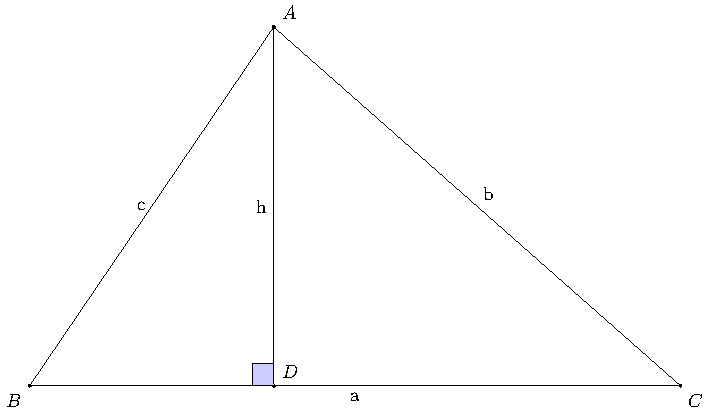
\includegraphics[width=0.6\columnwidth]{figs/trig_id/right/tri_sss.pdf}}
	\end{center}
	\caption{Area of a Triangle}
	\label{fig:tri_sss}	
\end{figure}

\solution We have
%
\begin{equation}
ar\brak{\Delta ABC} = \frac{1}{2}ah = \frac{1}{2}ab\sin C \quad \brak{\because \quad h = b \sin C}.
\label{eq:tri_area_sin}
\end{equation}

\item
	Show that 
	\begin{equation}
	\frac{\sin A}{a} = \frac{\sin B}{b} = \frac{\sin C}{c}
	\end{equation}

\solution 
\figref{fig:tri_sss} can be suitably modified to obtain 
\begin{align}
ar\brak{\Delta ABC} = 
\frac{1}{2}ab\sin C = \frac{1}{2}bc\sin A = \frac{1}{2}ca\sin B
	\label{tri:area-sin}
\end{align}
Dividing the above by $abc$, we obtain
	\begin{equation}
\label{eq:tri_sin_form}
	\frac{\sin A}{a} = \frac{\sin B}{b} = \frac{\sin C}{c}
	\end{equation}
This is known as the sine formula.	
%
\item 
	In \figref{fig:tri_isoc}, $AB = AC$.  Show that 
\begin{align}
	\angle B
	= \angle C 
\end{align}
\begin{figure}[H]
	\centering
		{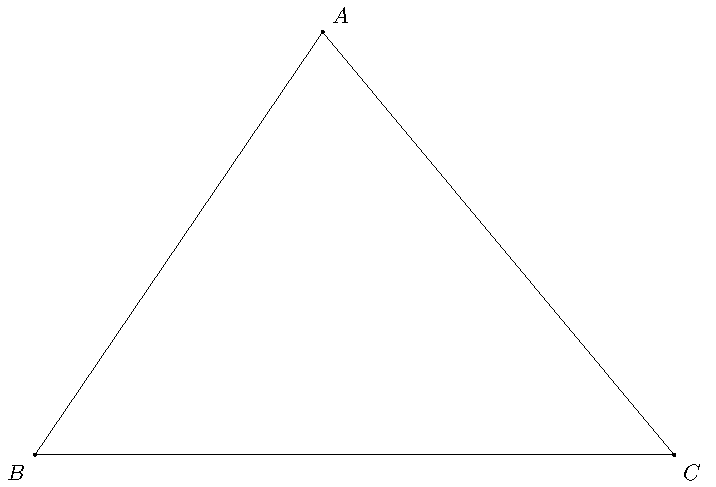
\includegraphics[width=0.6\columnwidth]{figs/trig_id/right/tri_isoc.pdf}}
	\caption{}
	\label{fig:tri_isoc}
\end{figure}
\solution Using the sine formula, 
\begin{align}
	\frac{AB}{\sin C}
	&=\frac{AC}{\sin B}
	\\
	\implies \sin B &= \sin C
	\text{ or, } \angle B = \angle C.
\end{align}
%\end{enumerate}
\item
In Fig. \ref{fig:tri_cosine_formula}, show that
%
\begin{equation}
\label{eq:tri_cos_mat}
\begin{pmatrix}
0 & c & b \\
c & 0 & a \\
b & a & 0
\end{pmatrix}
\begin{pmatrix}
\cos A \\
\cos B \\
\cos C
\end{pmatrix}
= 
\begin{pmatrix}
a\\
b\\
c
\end{pmatrix}
\end{equation}
%
%
\begin{figure}[!ht]
	\begin{center}
		
		%\includegraphics[width=0.6\columnwidth]{figs/ch2_triang_ar}
		%\vspace*{-10cm}
		{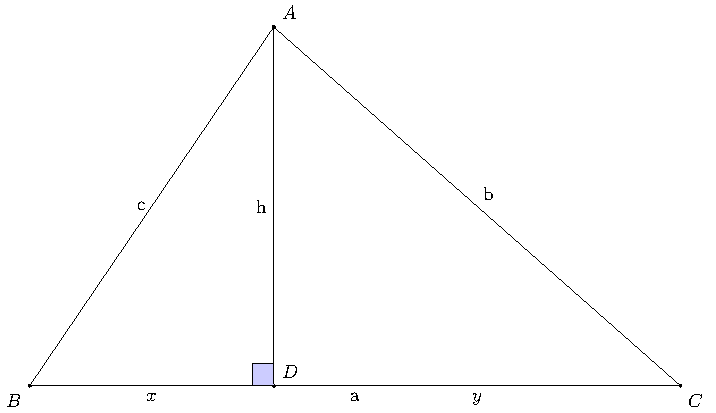
\includegraphics[width=0.6\columnwidth]{figs/trig_id/sincos/tri_cosine_formula.pdf}}
	\end{center}
	\caption{The cosine formula}
	\label{fig:tri_cosine_formula}	
\end{figure}
\solution From Fig. \ref{fig:tri_cosine_formula}, 
%
\begin{align}
	a = x + y &= b \cos C + c \cos B = \myvec{  \cos C & \cos B } \myvec{ b \\ c }
	\\
&=\myvec{0 & b & c } \myvec{ \cos A \\ \cos C \\ \cos B } 
\end{align}
%
Similarly,
%
\begin{align}
b &= c \cos A + a \cos C 
=\myvec{c & 0 & a } \myvec{ \cos A \\ \cos C \\ \cos B } 
	\\
c &= b \cos A + a \cos B
=\myvec{b & a & 0 } \myvec{ \cos A \\ \cos C \\ \cos B } 
\end{align}
%
The above equations can be expressed in matrix form as
\eqref{eq:tri_cos_mat}.

\item Show that 
\begin{equation}
\label{eq:tri_cos_form}
\cos A = \frac{b^2+c^2-a^2}{2bc}
\end{equation}
%
\solution 
Using the properties of determinants,
%
\begin{align}
\cos A = \frac{
\begin{vmatrix}
a & c & b \\
b & 0 & a \\
c & a & 0
\end{vmatrix}
	}
	{
\begin{vmatrix}
0 & c & b \\
c & 0 & a \\
b & a & 0
\end{vmatrix}
	}
	=\frac{ab^2 + ac^2 - a^3}{abc + abc} 
= \frac{b^2 + c^2 - a^2}{2abc}
\end{align}
%
\item Find Hero's formula for the area of a triangle.
\\
\solution 
From \eqref{prob:tri_area_sin}, the area of $\triangle ABC$ is 
\begin{align}
\label{eq:tri_geo_area_sin_form}
 \frac{1}{2}ab\sin C
%\\
&=\frac{1}{2}ab\sqrt{1-\cos^2C} 
\quad \brak{\text{from } \eqref{eq:tri_sin_cos_id}
%\eqref{eq:tri_geo_baudh}
}
\\
&=\frac{1}{2}ab\sqrt{1-\brak{\frac{a^2+b^2-c^2}{2ab}}^2} \brak{\text{from } \eqref{eq:tri_cos_form}
}
\\
&=\frac{1}{4}\sqrt{\brak{2ab}^2-\brak{a^2+b^2-c^2}}
\\
&=\frac{1}{4}\sqrt{\brak{2ab+a^2+b^2-c^2}\brak{2ab-a^2-b^2+c^2}}
\\
&= \frac{1}{4}\sqrt{\cbrak{\brak{a+b}^2-c^2}\cbrak{c^2-\brak{a-b}^2}}
\\
&= \frac{1}{4}\sqrt{\brak{a+b+c}\brak{a+b-c}\brak{a+c-b}\brak{b+c-a}}
\label{eq:tri_ex_hero_temp}
\end{align}
Substituting 
%
\begin{align}
s=\frac{a+b+c}{2}
\end{align}
%
in \eqref{eq:tri_ex_hero_temp}, the area of $\triangle ABC$ is 
%
\begin{align}
\label{eq:tri_area_hero}
\sqrt{s\brak{s-a}\brak{s-b}\brak{s-c}}
\end{align}
%
This is known as Hero's formula.
\item Show that 
%
\begin{align}
\label{eq:trig_id_sin_inc}
\alpha > \beta \implies \sin \alpha > \sin \beta
\end{align}
%

\begin{figure}[!ht]
	\begin{center}
		
		%\includegraphics[width=\columnwidth]{figs/fig:tri_sin_inc}
		%\vspace*{-10cm}
		{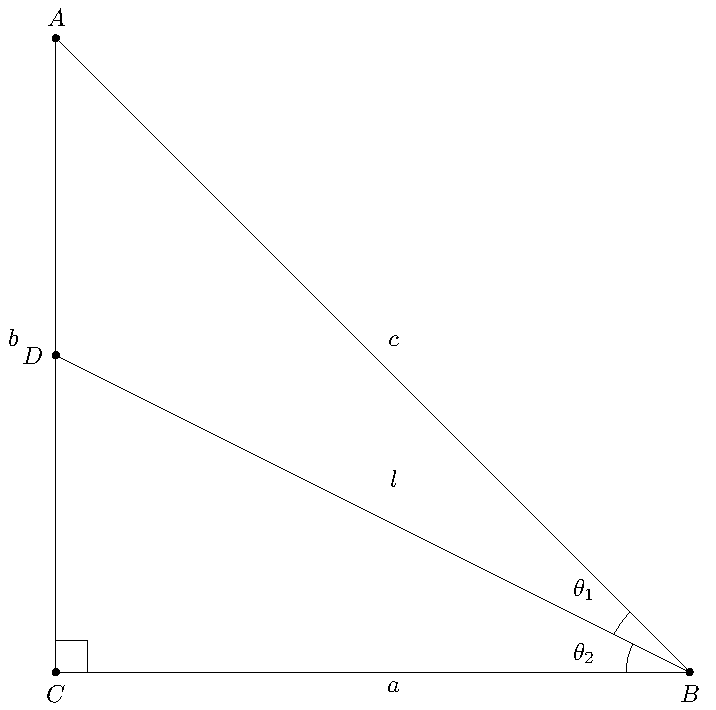
\includegraphics[width=0.6\columnwidth]{figs/trig_id/sincos/tri_sin_inc.pdf}}
	\end{center}
	\caption{}
	%\caption{$\sin \brak{\theta_1+\theta_2} = \sin\theta_1\cos\theta_2 + \cos\theta_1\sin\theta_2$}
	\label{fig:tri_sin_inc}	
\end{figure}
\solution In Fig. \ref{fig:tri_sin_inc}, 	
%
\begin{align}
ar\brak{\triangle ABD} &< ar \brak{\triangle ABC}
\\
\implies \frac{1}{2}lc \sin \theta_1 &<  \frac{1}{2}ac \sin \brak{\theta_1 + \theta_2 }
\\
\implies \frac{l}{a} &< \frac{\sin \brak{\theta_1 + \theta_2 }}{\sin \theta_1}
\\
\text{or, } 1 < \frac{l}{a} &< \frac{\sin \brak{\theta_1 + \theta_2 }}{\sin \theta_1}
\end{align}
%
from Theorem \ref{them:hyp_largest}, yielding 
\begin{align}
\implies \frac{\sin \brak{\theta_1 + \theta_2 }}{\sin \theta_1} > 1.
\end{align}

This proves \eqref{eq:trig_id_sin_inc}.
\end{enumerate}

